\begin{refsection}
    \renewcommand{\thefigure}{\arabic{figure}}
    \renewcommand{\thetable}{\arabic{table}}
    \renewcommand{\thequadro}{\arabic{quadro}}

    \chapter[Contribuições do Software GeoGebra para o ensino aprendizagem de função polinomial do 2º grau]{CONTRIBUIÇÕES DO SOFTWARE GEOGEBRA\footnote{GeoGebra é marca registrada do GeoGebra Institute ou GeoGebra, Inc.} PARA O ENSINO APRENDIZAGEM DE FUNÇÃO POLINOMIAL DO 2º GRAU}
    \label{chap:contrib-geogebra}
    
    \articleAuthor
    {Sarah Mara Silva Leôncio}
    {Licenciada e Bacharela em Matemática, Mestra em Ensino de Ciências Naturais pela UFRN e Especialização em Educação Matemática pelo IFESP. Professora na rede Estadual do RN e Município de Parnamirim. ID Lattes: 6902.2994.4515.2240. E-mail: legalmentemorena@hotmail.com.}

    \articleAuthor
    {Maria José Lima dos Santos}
    {Graduação em Matemática pela Universidade Federal do Rio Grande do Norte, Mestra em Sistemas e Computação e Especialização em Engenharia de Sistemas pela Universidade Federal do Rio Grande do Norte. MBA em Administração Pública e Especialista em Educação a Distância. Professora formadora no Instituto de Educação Superior Kennedy (IFESP --- SEEC). ID Lattes: 6234.8999.1285.9489. E-mail: mjlima@ifesp.edu.br.}
    
    \begin{galoResumo}
        \marginpar{
            \begin{flushleft}
            \tiny \sffamily
            Como referenciar?\\\fullcite{SelfLeôncioAndSantos2021Contribuições}\mybibexclude{SelfLeôncioAndSantos2021Contribuições}, p. \pageref{chap:contrib-geogebra}--\pageref{chap:contrib-geogebraend}, \journalPubDate{}
            \end{flushleft}
        }
        O presente artigo aborda uma pesquisa de caráter investigativo que teve como objetivo analisar as potencialidades do software GeoGebra como recurso de ensino e aprendizagem de quando se é estudado a construção de gráfico da função polinomial do 2º grau. A pesquisa realizada se justifica pelo fato de que o conceito de função polinomial se faz presente tanto no cotidiano dos discentes como em fenômenos associados a outras ciências. Por meio deste trabalho, observamos a importância do uso de recursos digitais para a compreensão dos conceitos matemáticos de forma motivadora, criativa e dinâmica.
    \end{galoResumo}
    
    \galoPalavrasChave{Gráficos. Função polinomial do 2º grau. GeoGebra.}
    
    \begin{otherlanguage}{english}
    
    \fakeChapterOneLine
    {GeoGebra Contributions for teaching\-{}-learning of quadratic functions}
    
    \begin{galoResumo}[Abstract]
        This article addresses an investigative research that aimed to analyze the potential of the GeoGebra software as a teaching and learning resource when studying the construction of graphs of second-degree polynomial functions. The research carried out is justified by the fact that the concept of polynomial function is present both in students' daily lives and in phenomena associated to other sciences. Through this work, we observe the importance of using digital resources to understand mathematical concepts in a motivating, creative and dynamic way.
    \end{galoResumo}
    
    \galoPalavrasChave[Keywords]{Graphs. Second-degree polynomial function. GeoGebra.}
    \end{otherlanguage}
    
    % \flourish

    \section{Introdução}

    Atualmente, um dos grandes obstáculos a ser enfrentado pelos professores de qualquer área do conhecimento é saber motivar os discentes, criar neles o gosto e a curiosidade para aprender. No componente curricular Matemática não é diferente, e em virtude disso, pesquisadores da Educação Matemática apresentam novas metodologias a fim de contribuir para o ensino e aprendizagem dos discentes. Entre estas metodologias podemos apresentar as Novas Tecnologias da Informação e Comunicação (NTIC) que vêm assumindo grande valia no meio educacional.  

    A Base Nacional Comum Curricular (BNCC), por exemplo, orienta em uma de suas competências a utilização das tecnologias digitais “para modelar e resolver problemas cotidianos, sociais e de outras áreas de conhecimento, validando estratégias e resultados”. \cite[p.~267]{DocumentoInstitucional2016Base}. Diante disso, o uso das NTICs na educação, além de possibilitar o ensino da Matemática mais prazeroso e divertido, contribui para elevar a sua qualidade da aprendizagem. Mas, para que isso seja efetivado, há a necessidade de que os professores tenham domínio e conhecimento destes recursos.  Além disso, como enfatiza \textcite[p.~102]{CARNEIROAndoAndPASSOS2014utilização} “O papel do professor nesse ambiente é de fundamental importância, porque somente a introdução dos computadores nas escolas não provoca mudanças nas práticas docentes enraizadas e no processo de ensino e de aprendizagem” 

    Desta forma, compreendemos que para que haja efetiva aprendizagem, necessitamos não somente dos recursos tecnológicos, mas de uma formação qualificada e continuada dos docentes que atuam nas escolas. Também há a necessidade de uma reflexão quanto ao uso destes recursos, pois de acordo com \textcite[p.~105]{CARNEIROAndoAndPASSOS2014utilização}, estes recursos devem possibilitar o interesse dos discentes pelas aulas e consequentemente motivá-los, modernizando o ambiente de sala de aula, facilitando a realização de tarefas, além de criar novas dinâmicas educativas.       

    Entre os recursos que o professor de matemática pode trabalhar na sala de aula, podemos citar: jogos online, softwares como o Poly, GeoGebra, Cabri, planilhas no Excel, Redes Sociais etc. Assim, diante desta apresentação, surgiram as seguintes questões: Por que utilizar recursos tecnológicos nas aulas de matemática? Que potencialidades o uso do software GeoGebra possibilita ao ensino-aprendizagem de Função Polinomial do 2º grau? Aulas utilizando recursos tecnológicos motivam os discentes para a aprendizagem dos conteúdos matemáticos? Quais vantagens o software GeoGebra possibilita aos professores de matemática? 

    Para responder estes questionamentos, o presente trabalho tem o propósito de investigar as potencialidades do software GeoGebra como recurso de ensino e aprendizagem quando se trata da construção de gráficos da Função Polinomial do 2° grau. Desta forma, para alcançar este objetivo, visamos investigar o grau de envolvimento dos discentes quando aplicamos atividade com o uso do software de geometria dinâmica. 



    \section{Referencial teórico}

    O século XXI é marcado por uma sociedade em que o fluxo de informação é abundante, de fácil acesso e que está em constante transformação. Em parte devemos essa situação ao fato de que a sociedade atual está submersa nas tecnologias da informação, que têm assumido uma relevância dentro do cenário educacional, em particular no processo de ensino-aprendizagem. Diante disto, e por meio de políticas públicas voltadas para a educação, houve a necessidade de se investir em recursos tecnológicos que contribuíssem tanto para o ensino e aprendizagem dos discentes, como também auxiliassem os professores durante suas aulas.  

    Entre estas políticas públicas podemos citar o Programa Nacional de Tecnologia Educacional (PROINFO), cuja finalidade é informatizar as escolas públicas de todo o país, seja rede estadual ou municipal, por meio da criação de laboratórios de informática. Estes laboratórios possibilitam aos professores, em particular os de matemática, uma proposta metodológica inovadora, como expressa \textcite[p.~20]{ROCHAAndPOFFALAndMENEGHETTI2015Utilização}: 

    \begin{quotation}
        Nas últimas décadas, o ensino da Matemática no Brasil vem apresentando progressos importantes com propostas de novas metodologias como a utilização de jogos educativos, materiais concretos, pesquisas que visam relacionar a matemática com o cotidiano dos alunos, além de softwares especialmente desenvolvidos para este fim.
    \end{quotation}

    Nesta perspectiva, por meio destes recursos, o aprender matemático torna-se mais atrativo e motivador aos discentes. Os próprios PCNs \cite{DocumentoInstitucional2006Parâmetros} afirmam que: 

    \begin{quotation}
        No uso de tecnologias para o aprendizado da Matemática, a escolha de um programa torna-se um fator que determina a qualidade do aprendizado. É com a utilização de programas que oferecem recursos para a exploração de conceitos e ideias matemáticas que está se fazendo um interessante uso de tecnologia para o ensino da matemática \cite[p.~89]{DocumentoInstitucional2006Parâmetros}. 
    \end{quotation}

    Entre os recursos metodológicos citados acima, os softwares têm contribuído de forma significativa para o ensino e aprendizagem dos alunos do século XXI. Os estudos e pesquisas no campo da Educação Matemática revelam que há diversos softwares que direcionam o ensino e a aprendizagem da Matemática no campo da geometria ou álgebra, dentre eles podemos citar: Cabri, Poly, GeoGebra, Maple, Sage, Matlab, entre outros. 

    A exemplo destes, temos o software de geometria dinâmica GeoGebra, que foi criado pelo professor Markus Hohenwarter, da Universidade de Salzburg, com a finalidade de dinamizar o estudo da Matemática. O GeoGebra permite trabalharmos Geometria, Álgebra, Cálculo e Estatística em um mesmo ambiente interativo. Além disso, vale salientar que: 

    \begin{quotation}
        O software apresenta três diferentes janelas: gráfica, algébrica ou numérica, e a folha de cálculo. Elas permitem que os objetos matemáticos sejam vistos em três diferentes representações: graficamente (pontos, gráficos de funções), algebricamente (coordenadas de pontos, equações) e nas células da folha de cálculo \cite[p.~7020]{LOPESAndOLIVEIRAAndAMORIM2013uso}. 
    \end{quotation}

    Assim, por meio destas janelas de visualizações (Figura \ref{fig:geogebra-wind}) podemos observar as representações dos objetos matemáticos tanto na forma geométrica como algébrica, além de possibilitar representações em forma de animações.

    \begin{figure}[ht]%
        \centering%
        \caption{GeoGebra}%
        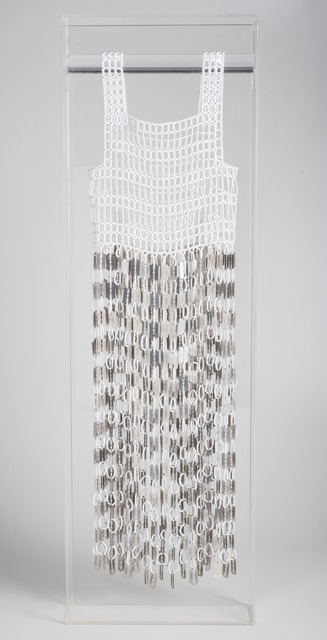
\includegraphics[width=.75\textwidth]{articles/03-contribuicoes-do-sof/image1.pdf}%
        \caption*{Fonte: Acervo da autora (2018).}%
        \label{fig:geogebra-wind}%
    \end{figure}%

    Atualmente, são várias as pesquisas voltadas para investigar as contribuições que o software GeoGebra tem possibilitado tanto no ensino básico como no superior. Entre os pesquisadores podemos citar \textcite{REISAndOZDEMIR2010UsingGeogebra}, \textcite{SHADAANAndEU2013Effec}, \textcite{BORBAAndPENTEADO2007Informática}. Estes defendem que o uso deste software durante as aulas de Matemática permite aos estudantes investigar, experimentar situações, conjecturar, usar sua criatividade além de motivá-los a aprender novos conceitos Matemáticos de forma dinâmica e interativa, de modo que:

    \begin{quotation}
        O software matemático GeoGebra pode beneficiar o processo de ensino e aprendizagem, conduzindo os estudantes por caminhos investigativos. Portanto, consideramos que o computador pode viabilizar a exploração de atividades diversas que podem ser bem enriquecedoras, por oferecer condições as múltiplas representações facilitando as conversões entre essas, onde permite a interatividade entre os objetos matemáticos e a visualização dos conceitos, possibilitando, assim, a formulação de conjecturas \cite[p.~201]{ARAUJOAndSILVA2015GeoGebra}. 
    \end{quotation}

    Além disso, \textcite[p.~571, tradução nossa]{REISAndOZDEMIR2010UsingGeogebra} observam o porquê de usar recursos como o GeoGebra nas aulas de matemática:  

    \begin{quotation}
        A matemática é vista como uma disciplina difícil pelos estudantes durante a vida educacional e seus modelos educacionais são amplamente discutidos (\textit{apud} Altun, 2008). Uma das razões dessas dificuldades são os conceitos abstratos que constituem essa disciplina. A fim de superar essas dificuldades, o uso da visualização ajuda a envolver os alunos, a chamar atenção deles, demonstra como a matemática é relevante para a vida deles e explica como os conceitos matemáticos funcionam (\textit{apud} Murphy, 2009). Desta forma, o resultado das ferramentas da tecnologia da informação no exercício da matemática é contextualizado. 
    \end{quotation}

    Diante das abordagens teóricas até agora apresentadas, o presente trabalho objetiva analisar as contribuições que este software pode trazer para o ensino e aprendizagem de funções, em particular, as Função Polinomial do 2º grau, já que o estudo de funções é um dos temas muito importantes a ser abordado durante o Ensino Médio e que está totalmente relacionado com o cotidiano dos discentes. Além disso, vale salientar que trabalhar este conteúdo apenas utilizando os recursos e métodos convencionais que associam as aulas expositivas com quadro e giz, limita a compreensão de conceitos e a visualização dos objetos Matemáticos. 

    \section{Discussão e métodos}

    Apresentamos nesta sessão uma experiência vivenciada durante as aulas de matemática no Laboratório de Informática da Escola Estadual Edgar Barbosa (Figura \ref{fig:ee-edgar-b}), em específico, nas cinco turmas de 1\textsuperscript{as} séries do Ensino Médio, no qual utilizamos como recurso tecnológico o software GeoGebra para auxiliar nas construções dos gráficos das Funções Polinomiais do 2º grau.

    \begin{figure}[ht]%
        \centering%
        \caption{Escola Estadual Edgar Barbosa}%
        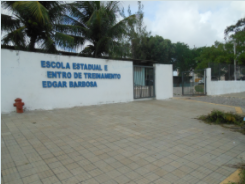
\includegraphics[width=.50\textwidth]{articles/03-contribuicoes-do-sof/image2.png}%
        \caption*{Fonte: Repositório Digital do PIBID.}%
        \label{fig:ee-edgar-b}%
    \end{figure}%

    Atualmente o laboratório de informática da escola (Figura \ref{fig:lab-ee-edgar-b}) é constituído por uma sala climatizada contendo 16 (dezesseis) notebooks, uma bancada de mármore, cadeiras, lousa interativa e um multimídia. Este espaço é frequentemente utilizado pelos professores da escola para ministrar aulas interativas nas áreas de Biologia, Química, Física, Educação Física e Matemática, como também, para que os discentes possam realizar pesquisas.

    \begin{figure}[ht]%
        \centering%
        \caption{Laboratório}%
        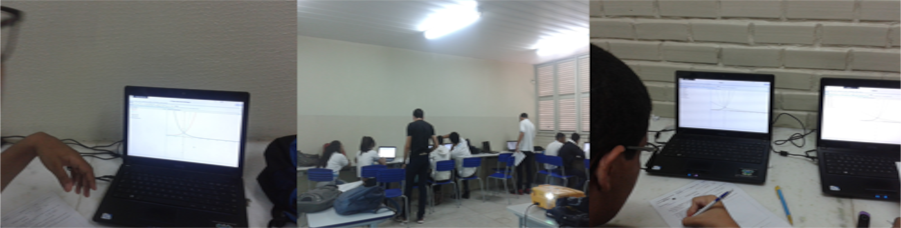
\includegraphics[width=.90\textwidth]{articles/03-contribuicoes-do-sof/image3.png}%
        \caption*{Fonte: Acervo da autora (2018).}%
        \label{fig:lab-ee-edgar-b}%
    \end{figure}%

    Iniciamos, a princípio, apresentando aos discentes o software GeoGebra, que foi utilizado como recurso metodológico para construção de gráficos de funções. Durante este momento, os discentes tiveram a oportunidade de manuseá-lo e conhecer as ferramentas disponíveis no software, para em seguida trabalharmos os gráficos vistos em sala de aula. Portanto, ao iniciarmos nossa pesquisa, usamos como estratégia, as aulas expositivas na sala de aula com construção de gráficos feitos pelos alunos e, em seguida, aulas no laboratório, utilizando as atividades de Função Polinomial do 2º grau. Tomamos como base as atividades propostas no livro didático adotado pela escola, \textcite{DANTE2016Matemática} e \textcite{BALESTRI2016Matemática} porque estes já trazem atividades que já sugerem e orientam o uso do GeoGebra como ferramenta para estudo da construção, comportamento e análise de gráficos. 

    Assim, durante este período foi introduzida a definição de Função Polinomial do 2º grau presente no livro didático: \textit{``Uma função $f: \mathbb{R} \rightarrow \mathbb{R}$ chama-se função quadrática quando existem números reais $a$, $b$ e $c$, com $a \neq 0$, tal que $f$ leva $x$ em {\boldmath$ax^2 + bx + c$}, para todos $x \in \mathbb{R}$.''} \cite[p.~102]{DANTE2016Matemática}.  

    Para familiarizar os discentes com a função, foi apresentado um exercício com várias Funções do 2º grau cuja finalidade era identificar os parâmetros $a$, $b$ e $c$. Em seguida, orientamos e ensinamos aos discentes a fazer o cálculo da imagem da função para os valores atribuídos à variável $x$. Dando continuidade ao estudo, foram abordados os conceitos de raízes da função e pontos de interseção, bem como a resolução de problemas envolvendo Função Polinomial do 2º grau, até darmos início ao estudo dos seus gráficos. 

    Com a desenvoltura do processo, trabalhamos en três momentos distintos a construção dos gráficos da função polinomial. A saber, no primeiro momento introduzirmos gráfico de função por meio das tabelas, isto é, dados os valores da abscissa os discentes determinavam a imagem da função e, em seguida, apresentariam as coordenadas do ponto no plano cartesiano para poderem formar o gráfico da função polinomial do 2º grau. O segundo momento, após termos trabalhado os conceitos de parâmetros, discriminante, ponto máximo e mínimo, vértice do gráfico, concavidade da parábola, passamos a trabalhar com os discentes a construção dos gráficos utilizando estes conceitos. No último momento, com os discentes já familiarizados com as ferramentas do GeoGebra, demos início ao estudo dos gráficos de Função Polinomial do 2º grau, agora com um olhar investigativo. 

    Os três momentos possibilitaram uma investigação da relação entre o pensamento geométrico e algébrico feita pelos discentes. No primeiro momento em que abordados a construção dos gráficos por meio das tabelas, os discentes observaram que os gráficos estavam limitados a quantidade de pontos apresentados e que este processo, dependendo da quantidade de pontos ou do campo de visão do gráfico, limita a visualização do comportamento geométrico da função.  

    Já o segundo momento possibilitou aos discentes visualizarem o comportamento geométrico do gráfico da função de uma maneira mais ampla, já que este procedimento exigiu dos discentes o conhecimento de vários conceitos presentes no estudo do gráfico da Função Polinomial do 2º grau. Entretanto, para a diversidade de comportamentos de gráficos e o curto período de tempo presente na sala de aula ou até mesmo erros algébricos apresentados pelos alunos torna este método limitado. Todavia, a conexão dos métodos empregados nos três momentos tornou o ambiente de aprendizagem enriquecedor, conforme foi observado durante esta investigação em sala de aula. A seguir descrevemos os três momentos e as atividades desenvolvidas com os discentes:
    
    \paragraph{1º momento} Nesta perspectiva, iniciamos nosso percurso apresentando aos discentes algumas Funções Polinomiais do 2º grau e que a partir delas, eles poderiam atribuir valores para abcissa e determinar suas respectivas ordenadas, consequentemente, as coordenadas dos pontos. Posteriormente, teriam o papel de identificar no plano cartesiano os pontos e em seguida traçar o gráfico. A atividade apresentada continha as seguintes funções:
    \begin{itemize}
        \item $f(x) =  x^2 - 7x + 10$
        \item $f(x) =  x^2 - 6x +  9$
        \item $f(x) =  x^2 - 2x +  2$
        \item $f(x) = -x^2 + 2x +  3$
    \end{itemize}
    Cujos respectivos gráficos apresentariam comportamentos conforme observamos nas Figura \ref{fig:graficos-geogebra}:

    \begin{figure}
        \centering%
        \caption{Gráficos das funções}%
        \begin{tabular}{cc}%
            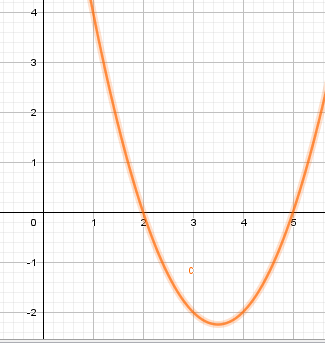
\includegraphics[width=35mm]{articles/03-contribuicoes-do-sof/image4.png}%
            & 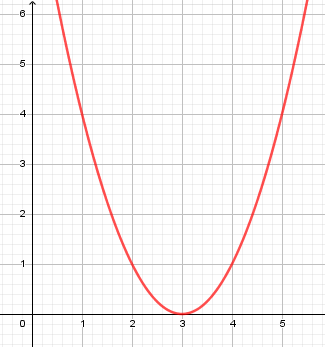
\includegraphics[width=35mm]{articles/03-contribuicoes-do-sof/image5.png}\\%
            (a) $f(x) = x^2 - 7x + 10$ & (b) $f(x) = x^2 - 6x +  9$ \\[2ex]%
            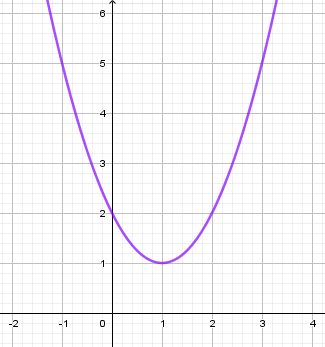
\includegraphics[width=35mm]{articles/03-contribuicoes-do-sof/image6.png}%
            & 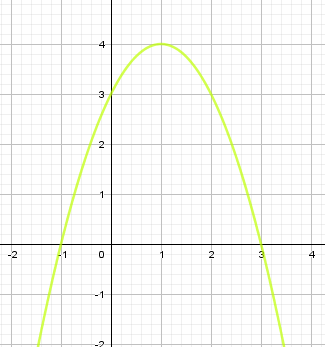
\includegraphics[width=35mm]{articles/03-contribuicoes-do-sof/image7.png}\\%
            (c) $f(x) = x^2 - 2x + 2$ & (d) $f(x) = -x^2 + 2x +  3$ \\%
        \end{tabular}%
        \caption*{Fonte: \textit{Printscreen} dos gráficos no GeoGebra.}%
        \label{fig:graficos-geogebra}%
    \end{figure}

    Estas funções foram escolhidas intencionalmente com aparentes comportamentos distintos, com a finalidade que os discentes fizessem a construção dos gráficos, observando e comparando o comportamento da parábola em cada situação representada. 

    Assim, para a construção dos gráficos, os alunos foram orientados a preencher uma tabela que continha os valores de $x$, mas que deveriam ser calculados os valores da imagem, isto é, $f(x)$. Ao formar as coordenadas dos pontos, eles poderiam traçar o gráfico (fazer a representação gráfica) de cada função dada. Este gráfico era formado por nove pontos, como podemos observar na Figura \ref{fig:atividade}.
    
    \begin{figure}[ht]%
        \centering%
        \caption{Atividade}%
        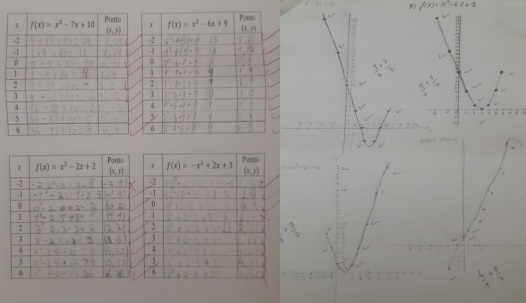
\includegraphics[width=.80\textwidth]{articles/03-contribuicoes-do-sof/image8.jpeg}%
        \caption*{Fonte: Acervo da autora (2018).}%
        \label{fig:atividade}%
    \end{figure}%

    As Figuras \ref{fig:atividade} e \ref{fig:atividade-2} representam os cálculos e a representação gráfica apresentados pelos alunos.

    \begin{figure}[ht]%
        \centering%
        \caption{Atividade}%
        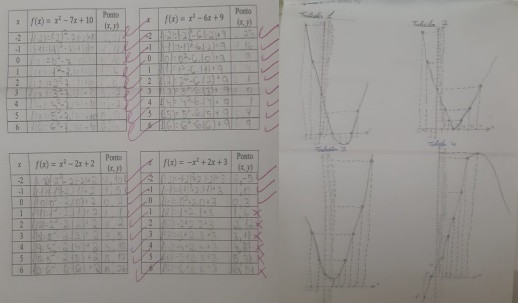
\includegraphics[width=.80\textwidth]{articles/03-contribuicoes-do-sof/image9.jpeg}%
        \caption*{Fonte: Acervo da autora (2018).}%
        \label{fig:atividade-2}%
    \end{figure}%

    Nos cálculos realizados, observamos situações diversas de confusão em relação à identificação das coordenadas, por exemplo, trocavam a ordem do $x$ por $y$, erros cometidos no cálculo da imagem prejudicavam a construção do gráfico, e isso foi notável para construção do gráfico da função $f(x)= -x^2 + 2x + 3$, cuja concavidade da parábola é voltada para baixo, mas a maioria dos alunos esboçaram a concavidade voltada para cima, desconsiderando a regra para o cálculo da potência.

    Ao analisar este primeiro momento, observamos que neste caso o método não traz resultados satisfatórios para o estudo do comportamento do gráfico de uma Função do 2º grau, pois existem erros recorrentes da aritmética resultantes de operações matemáticas quando se há necessidade da análise de sinal, valores da imagem, troca dos valores da abscissa com ordenadas, identificação do ponto no plano cartesiano resultam no erro da construção dos gráficos, pois neste momento supomos que os discentes não tinham conhecimento dos conceitos referentes aos parâmetros, concavidade, vértice e ponto de máximo e mínimo, consequentemente, não possuem a sensibilidade de julgar o gráfico elaborado pelas coordenadas atribuídas por eles. 

    Além disso, o aluno limita a construção dos gráficos apenas aos pontos dados, prejudicando a visualização do comportamento do gráfico, a saber, visualizar vértice, raízes e interseção com eixo $y$. Apesar disso, os discentes argumentam preferir construir os gráficos utilizando tabela, porque acham menos trabalhoso em relação aos cálculos presentes no segundo momento, como veremos a seguir. 

    \paragraph{2º momento} No segundo momento, após apresentarmos aos discentes o gráfico de uma Função Polinomial do 2º grau, trabalhamos com eles os conceitos de parâmetro, raízes da função, os valores do discriminante, eixo de simetria, vértice e valores de máximo e mínimo, propusemos aos alunos atividades que eles pudessem construir os gráficos desta função usando estes conceitos. 

    Desta forma, ao falar de parâmetro, os discentes deveriam estar cientes que o parâmetro $a$ identifica se a concavidade da parábola estará voltada para cima ou para baixo, como também fala sobre a abertura da parábola, o parâmetro $b$ indica se a parábola irá interceptar o eixo $y$ na parte crescente ou decrescente e o parâmetro $c$ expressa o valor em que a parábola irá interceptar o eixo $y$. Em relação ao discriminante, para $\Delta > 0$, a função apresentará duas raízes reais e distintas, ou seja, o gráfico interceptará o eixo $x$ em dois pontos de coordenadas $(x_1, 0)$ e $(x_2, 0)$; para $\Delta = 0$ a função terá duas raízes reais e iguais, ou seja, o gráfico da função intercepta o eixo $x$ em um único ponto; e para $\Delta < 0$, a função não apresenta raízes reais, isto é, o gráfico não irá interceptar o eixo das abscissas. Assim, para construir e analisar o comportamento do gráfico da função do 2º grau, os discentes deveriam ter conhecimento de todos estes conceitos.  

    Quando questionados em relação à atividade anterior, esta, na visão da grande maioria dos discentes é mais trabalhosa, pois requer que os estudantes usem todo embasamento teórico para a construção dos gráficos, conforme foi ensinado na sala de aula. Este embasamento teórico requer que os alunos saibam quando a concavidade da parábola está voltada para cima ou para baixo, se o gráfico da função irá interceptar o eixo da abscissa e em quais valores, os valores de máximo e mínimo da função. Enfim, estes cálculos contribuem para que o gráfico seja visualizado de uma maneira mais detalhada e de forma geral, contribuindo assim, para o sucesso na hora da elaboração dos gráficos. 
    
    Nesta atividade, os alunos identificaram onde o gráfico interceptaria o eixo $x$ e o eixo $y$, se a parábola estava voltada para cima ou para baixo, identificaram o eixo de simetria e os pontos máximo ou mínimo, resultando assim, em uma visão detalhada do comportamento do gráfico. Este método, apesar de ser trabalhoso, possibilita uma compreensão do comportamento do gráfico tornando menores os erros na hora de apresentar o gráfico, além de permitir ao aluno julgar a construção do gráfico por meio dos conceitos apresentados, como pode ser observado nas Figuras \ref{fig:atividade-3} e \ref{fig:atividade-4}.

    \begin{figure}[ht]%
        \centering%
        \caption{Atividade}%
        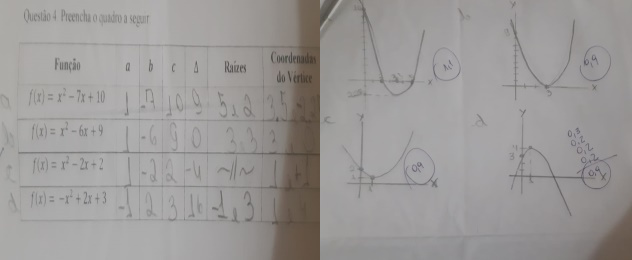
\includegraphics[width=.80\textwidth]{articles/03-contribuicoes-do-sof/image10.jpeg}%
        \caption*{Fonte: Acervo da autora (2018).}%
        \label{fig:atividade-3}%
    \end{figure}%

    \begin{figure}[ht]%
        \centering%
        \caption{Atividade}%
        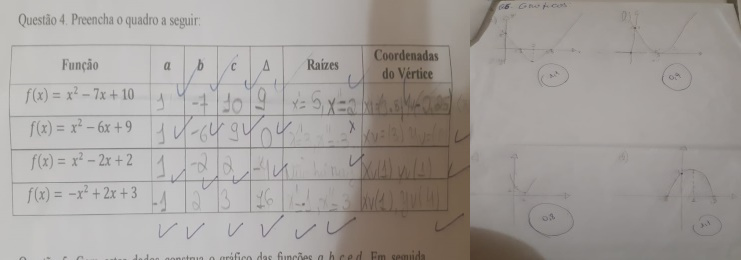
\includegraphics[width=.80\textwidth]{articles/03-contribuicoes-do-sof/image11.jpeg}%
        \caption*{Fonte: Acervo da autora (2018).}%
        \label{fig:atividade-4}%
    \end{figure}%

    Entretanto, apesar destes dois momentos apresentarem sua importância para o ensino e aprendizagem acerca do comportamento dos gráficos, eles requerem tanto do professor quanto dos alunos um maior tempo para que o estudo seja realizado. Há a necessidade da construção de vários gráficos para compreender o papel de cada conteúdo abordado, isto é, para um aluno compreender que o parâmetro $a$ identifica que a concavidade da parábola será voltada para cima ou para baixo, que os valores numéricos deste parâmetro influenciarão na abertura da parábola, necessitasse de atividades que requeiram a construção de vários gráficos para que eles possam assimilar a influência do parâmetro no comportamento do gráfico. 

    Assim, modificando os valores dos parâmetros $a$, $b$ e $c$, observamos que teremos uma determinada função polinomial do 2º grau que corresponderá a um determinado gráfico. Para observarmos o comportamento de diferentes funções há a necessidade de construir diferentes gráficos e analisar a influência do discriminante, dos valores dos parâmetros e raízes. Todavia, há um programa a ser seguido durante todo o ano letivo, assim, os docentes acabam limitando as variedades de exemplos que poderiam ser apresentados, tornando o trabalho do professor limitado a apresentar poucas funções. 

    Em oposição aos métodos de ensino expositivo, a saber, aqueles em que o professor e os discentes ficam limitados ao: quadro, projetores multimídia, aos livros e atividades didáticas; softwares como o GeoGebra abrangem novas possibilidades de ensino e aprendizagem, já que este ambiente interativo favorece o trabalho do professor na hora de ministrar os conteúdos relacionados a gráficos de função e possibilita a construção, a análise do comportamento dos gráficos e a compreensão dos conceitos abordados em sala de aula. 

    \paragraph{3º momento} O terceiro momento foi caracterizado por trabalharmos com os alunos a construção dos gráficos da Função Polinomial do 2º grau por meio do software GeoGebra. Inicialmente, os alunos conheceram o laboratório de informática da escola (Figura \ref{fig:atividade-5}) onde apresentamos o software, sua barra de ferramentas, comandos de entrada, as janelas algébrica, geométrica e os comandos que usaríamos para o estudo das funções. Assim, esta aula ficou voltada para que os discentes conhecessem e manipulassem as ferramentas do software GeoGebra.

    \begin{figure}[ht]%
        \centering%
        \caption{Atividade}%
        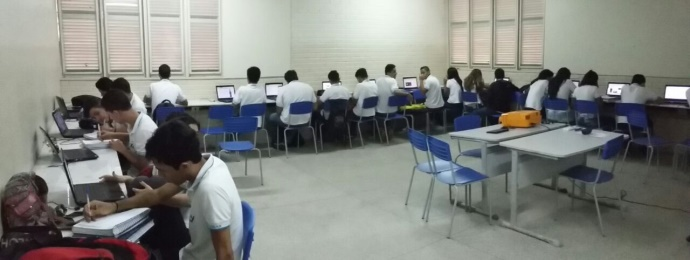
\includegraphics[width=.80\textwidth]{articles/03-contribuicoes-do-sof/image12.jpeg}%
        \caption*{Fonte: Acervo da autora (2018).}%
        \label{fig:atividade-5}%
    \end{figure}%

    Finalizada esta etapa, aplicamos atividades que abordavam a construção de gráficos usando o software GeoGebra. Iniciamos por uma atividade em que os alunos, utilizando o comando de entrada, digitavam a expressão algébrica da Função Polinomial do 2º grau e o software apresentava o desenho da parábola na janela geométrica, apresentava as raízes, o ponto de interseção com eixo y e o ponto que representava o vértice da parábola. Além disso, estes dados poderiam ser conferidos pelos discentes na janela algébrica. Feito isto, os discentes manualmente conferiram os dados apresentados pelo software utilizando os conceitos estudados em sala de aula (Figura \ref{fig:atividade-6}). 

    \begin{figure}[ht]%
        \centering%
        \caption{Atividade}%
        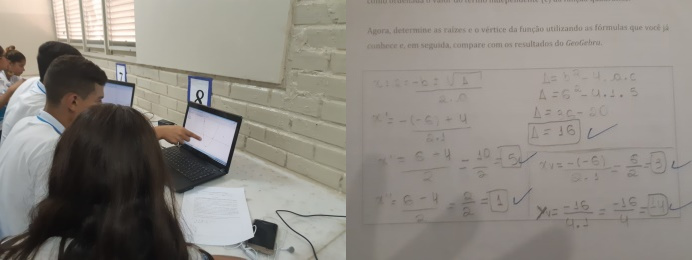
\includegraphics[width=.80\textwidth]{articles/03-contribuicoes-do-sof/image13.jpeg}%
        \caption*{Fonte: Acervo da autora (2018).}%
        \label{fig:atividade-6}%
    \end{figure}%

    A segunda atividade usando o GeoGebra (Figura \ref{fig:atividade-7}) constituía-sa em uma sequência de passos a ser realizada no software. Neste momento, foi utilizado o comando controle deslizante (ferramenta do GeoGebra que permite inserir uma variável que pode ser alterada utilizando o mouse) para representar os parâmetros $a$, $b$ e $c$ na função $f(x) = ax^2 + bx + c$ e que possibilitou aos discentes manipulá-los de tal forma que poderiam visualizar os efeitos dos valores dos parâmetros sobre o gráfico da função.

    \begin{figure}[ht]%
        \centering%
        \caption{Atividade}%
        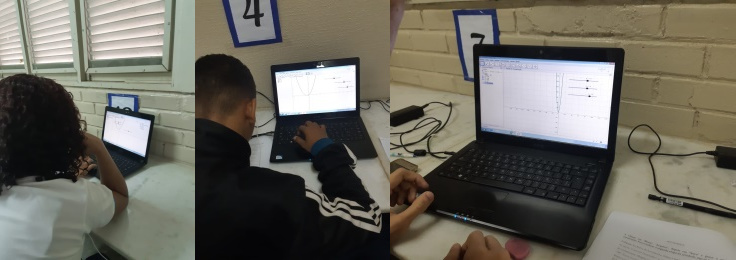
\includegraphics[width=.80\textwidth]{articles/03-contribuicoes-do-sof/image14.jpeg}%
        \caption*{Fonte: Acervo da autora (2018).}%
        \label{fig:atividade-7}%
    \end{figure}%

    Este momento possibilitou aos discentes, em um curto período de tempo, uma maior variedade de gráficos, contribuiu para que eles compreendessem os conceitos apresentados em sala de aula, como por exemplo, que a abertura e sentido da concavidade de uma parábola dependem dos valores do parâmetro $a$, que a interseção da parábola no eixo $y$ será no ramo crescente se valor do parâmetro $b$ for positivo e será no ramo decrescente se o valor de $b$ for negativo, e o parâmetro $c$ corresponde ao valor em que a parábola intersecta o eixo $y$. Possibilitou a visualização de gráficos no centro do eixo do plano cartesiano e também gráficos distantes deste eixo, permitindo visualizar pontos de intersecção, vértice e concavidade, além de identificar domínio e imagem deste tipo de função. 

    Enfim, as aulas ministradas no laboratório utilizando como recurso metodológico o software GeoGebra possibilitaram, tanto ao professor como aos discentes, várias oportunidades, pois usando este ambiente interativo, os discentes puderam fazer o estudo dos gráficos de forma dinâmica, possibilitando assim, plotar os gráficos de diferentes funções em um mesmo ambiente interativo, comparar e analisar o comportamento dos diversos gráficos em curto período de tempo. Desta forma, o uso deste software torna o ambiente de sala de aula motivador e enriquecedor. 

    Assim, ao solicitarmos para que os alunos descrevessem a importância do uso do software GeoGebra para o ensino aprendizagem da Matemática, destacamos três respostas entre tantas outras similares:
    \begin{quotation}
        \medskip\noindent{}Aluno A: “Utilizar mais o uso do GeoGebra, na minha opinião facilita para quem tem um baixo desenvolvimento em desenvolver um gráfico (tipos eu)\dots~Podemos utilizar da melhor forma e adquirir um nível de aprendizado.”

        \medskip\noindent{}Aluno B: “Eu acho que devemos continuar as aulas no laboratório com o GeoGebra, porque esse programa permite a criação de atividades que exploram diversos conteúdos matemáticos de maneira prática, instigante, dinâmica e eficiente no nosso aprendizado.” 
        
        \medskip\noindent{}Aluno C: “Eu acho que o uso do GeoGebra ajuda na parte da interpretação de um gráfico, já que muitos não conseguem fazê-los perfeitamente. Com o uso do aplicativo podemos assim trazer e resolver nossas dúvidas os gráficos onde não conseguimos representar.” 
    \end{quotation}
    Estas falas foram extraídas de uma enquete feita no grupo do WhatsApp da turma, conforme representadas na Figura \ref{fig:relatos-wpp}.

    \begin{figure}[ht]%
        \centering%
        \caption{Relatos do grupo do WhatsApp}%
        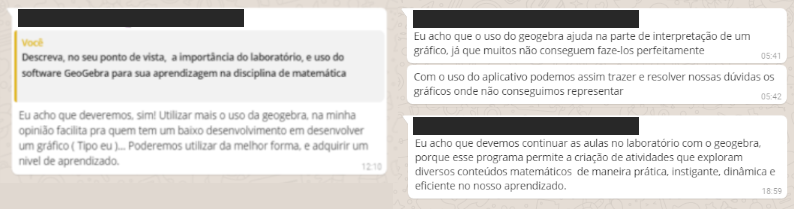
\includegraphics[width=.90\textwidth]{articles/03-contribuicoes-do-sof/image15.png}%
        \caption*{Fonte: Acervo da autora (2018).}%
        \label{fig:relatos-wpp}%
    \end{figure}%

    Entretanto, vale salientar que, assim como nos momentos anteriores, o uso desta ferramenta possui suas limitações, pontos negativos. Entre estes pontos, temos a própria estrutura do laboratório, pois são poucos os computadores para a quantidade de alunos por turma. Apesar de vivermos num ambiente em que a tecnologia se faz presente, ainda encontramos discentes que possuem dificuldades em manusear um computador. Em relação ao software, alguns estudantes argumentaram não saber manipular o GeoGebra e ter que ficar sempre pedindo ajuda da professora. Mas, tais limitações não superam a importância que este recurso traz para o ensino e aprendizagem de funções, pois manipular, visualizar, comparar e investigar possibilita o desenvolvimento de habilidades ao aluno tais como: a curiosidade, sensibilidade e autonomia.

    \section{Considerações finais}

    Aprender é um processo árduo que requer do sujeito interesse, força de vontade, motivação e curiosidade. Porém, nem sempre escolhemos aprender o que desejamos, mas somos levados a conhecer o que é necessário para nos tornarmos cidadãos críticos e conhecedores do mundo em que vivemos. Assim, nem tudo que aprendemos é porque queremos, mas porque se faz necessário. 

    Desta forma, a escola possui o papel de mediar o conhecimento gerado pela humanidade e os valores aplicados na sociedade. Isso provoca um choque no sujeito que está aprendendo, que se questiona: “onde usarei isto na minha vida?”. Que importância terá para este sujeito aprender a construir ou interpretar um gráfico? Como um professor de matemática poderá motivar estes discentes tornando sua aula mais atrativa? O mais importante ainda é: Como levá-lo a compreender, de forma significativa, aquilo que se é ensinado? São questões que são frequentemente levantadas pelos educadores e sujeitos da aprendizagem. 

    Foi com a intenção de motivar a aprendizagem de forma significativa que este trabalho analisou as contribuições que o software GeoGebra poderia trazer para o ensino e aprendizagem de funções do 2º grau por meio de atividades realizadas no laboratório da escola e na sala de aula. Assim, para atribuirmos a importância deste recurso metodológico para a sala de aula, optamos por trabalhar com os discentes três modos para o estudo do gráfico da função polinomial do 2º grau, a fim de compararmos os processos apresentados e acompanhar a desenvoltura dos alunos em relação a cada momento. 

    Compreendemos que cada momento teve sua importância, mas também as limitações no ensino-aprendizagem de funções polinomiais do 2º grau. Porém, o uso de recurso metodológico, como o software GeoGebra contribui de forma significativa para entender os conceitos relacionados à construção dos gráficos de uma função, em particular, as funções polinomiais do 2º grau. Isto porque o ambiente interativo do software possibilita verificar diferentes gráficos em mesmo sistema de eixo, o comportamento da função em relação aos seus parâmetros, identificar os conceitos de função abordados em sala de aula, além de, simplificar o tempo de abordagem do conteúdo. As aulas tornam-se atrativas, despertando nos discentes, a curiosidade, senso investigativo e desejo em aprender. 

    O uso deste recurso, em comparação com os momentos anteriores, foi bem-visto pelos discentes que argumentaram estar mais instigados, possibilitando aprender matemática de uma forma diferente, a tecnologia foi usada para algo produtivo, os discentes puderam interagir entre si por ser algo novo e diferente. Contribuiu para que a professora apresentasse o conteúdo de uma forma interativa inovadora. 

    Enfim, apesar das limitações detectadas durante o uso do GeoGebra nas atividades propostas, avaliamos que foi de fundamental importância compreender as estruturas das funções e observar que cada função possui um gráfico, suas características e comportamento que ficam mais interessantes de serem estudadas em um ambiente interativo. 

    \printbibliography[heading=subbibliography,notcategory=fullcited]

    \nocite{DocumentoInstitucional2006Orientações}
    \nocite{DocumentoInstitucional2017Escola}

    \label{chap:contrib-geogebraend}

\end{refsection}
